\documentclass[12pt,a4,english,finnish,pdflatex%,handout
]{beamer}
\definecolor{MyGreen}{RGB}{50, 120, 50}
\usecolortheme[named=MyGreen]{structure}

\usepackage{babel}
\usepackage[utf8]{inputenc}
\usepackage[T1]{fontenc}
\usepackage{amsmath,amssymb} 
\usepackage{animate}
\usepackage{multimedia}

\usepackage{natbib}
\bibpunct[: ]{(}{)}{,}{}{}{;}

\usepackage{tikz}

\usepackage{tipa}

\usepackage{hyperref}

\setbeamertemplate{navigation symbols}{}

\graphicspath{{figures/}}

\setlength{\leftmargini}{0pt}
\setlength{\leftmarginii}{1em}

\newcommand{\kommentti}[1]{
  {\bf[#1]}
}



\begin{document}
\title{Borrowing a Language 101} 
\author{Pertti Palo} \date{16 April 2022}

\frame{\titlepage
} 

\frame{\frametitle{Land acknowledgement}
We wish to acknowledge and honor the Miami, Delaware, Potawatomi, Kickapoo, and
Shawnee people, on whose ancestral homelands we are today and/or on whose
ancestral homelands I have worked on this presentation. 
}

\frame{\frametitle{Housekeeping and Warnings}
  \begin{itemize}
  \item I want to keep this a safe space of mutual respect.
  \item The organisers told me I should tell you, that I may swear during this
  presentation.
  \item Personally, I find it more important to give you a content warning
  concerning topics such as colonization, oppression, pejoratives, etc. 
  \end{itemize}  

  \vspace*{.5cm}

  \begin{itemize}
    \item Please feel free to ask questions at any point.
    \item There will also be time for discussion and questions afterwards. I do
    not intend to fill the full hour with just me talking.
  \end{itemize}
}


\frame{\frametitle{Outline}
  \begin{itemize}
  \item Today: Borrowing a Language 101
    \begin{itemize}
    \item Housekeeping and warnings
    \item Who am I and why am I here?
    \item Case study: Announ World
    \item Tentative principles for choosing languages
    \item Couple of things about language trees
    \item Some ideas to toss around
    \end{itemize}
  \item {\usebeamercolor[gray]{} Tomorrow: Ideas for Fantastic ((un)real) Speech}
  \begin{itemize}
    \item  {\usebeamercolor[gray]{} Dragon speech!}
    \item  {\usebeamercolor[gray]{} Bird people!}
    \item  {\usebeamercolor[gray]{} Speech and magic!}
  \end{itemize}
  \end{itemize}
}

\frame{\frametitle{Who's this guy?}
  \begin{columns}
    \begin{column}{5cm}
      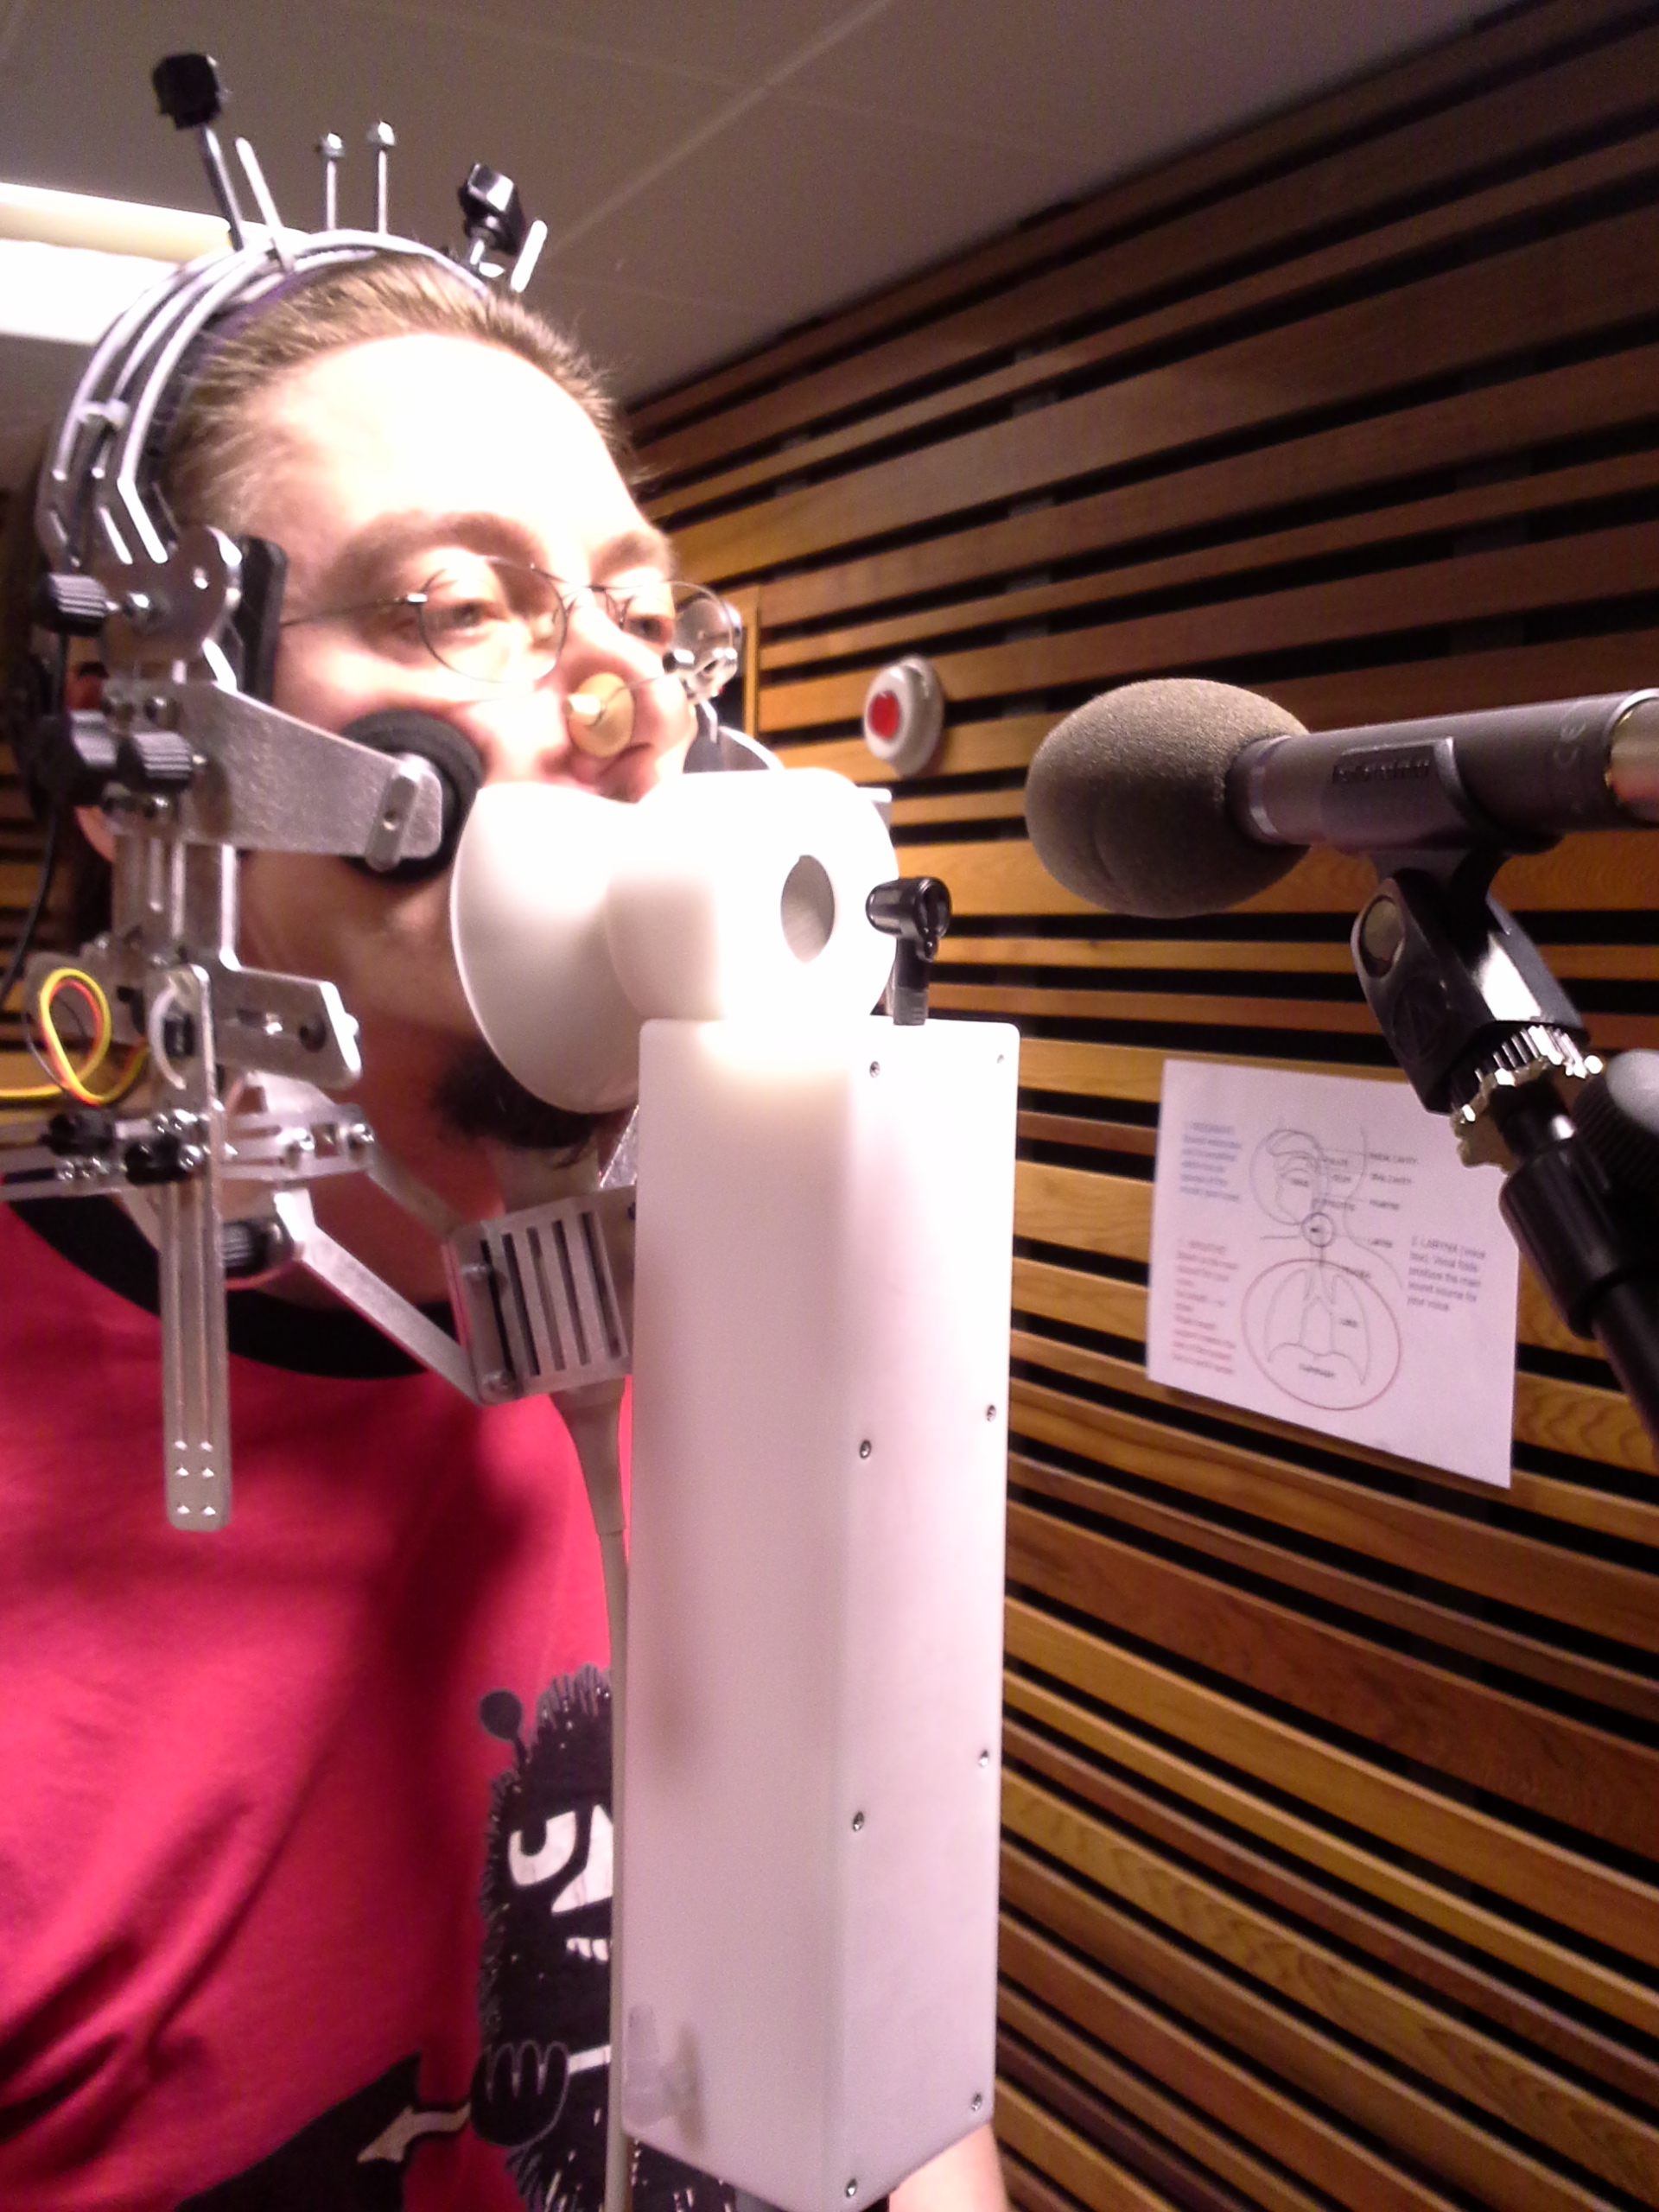
\includegraphics[width=\columnwidth]{uti_eva.png}
    \end{column}
    \begin{column}{5cm}
      \begin{itemize}
      \item Pertti Palo
      \item I've got a couple of degrees loosely speaking in engineering.
      \item I've also got a PhD in Phonetics.
      \item I have no formal qualifications in today's topic, but I do know a
      lot about speech production, but\ldots
      \end{itemize}
    \end{column}
  \end{columns}
} 

\frame{\frametitle{What lead me here?}
\begin{itemize}
  \item I am not a text linguist but rather a phonetician and a speech
  researcher.
  \item When I say 'language' I mainly mean spoken language today. 
  \item Besides a speech researcher with 20+ years of experience, I've been an
  RPG enthusiast for 30+ years. 
  \item Recently I've also started training as an oral storyteller which has
  some interesting connections with RPGs but also with science.
\end{itemize}
}

\frame{\frametitle{Announ (my world -- and multiverse)}

\begin{itemize}
  \item It all started with wanting to improve D\&D. 
  \item No, not the current one, the 1980's one. 
  \item Anyhow, I also had some very nice (Finnish) magazines with good
  adventures that I wanted to combine into an open ended campaign and for some
  reason decided against running it in any Known World. 
  \item So enter Announ World. 
  \begin{itemize}
    \item First drawn to the requirements of my campaign idea.
    \item Later expanded with help from
    the old world building mailing list (hello 90's), the MythoPoet sheets, and the
    excellent "Top Down and Bottom Up world designing" article. 
    \item I stole a good deal of the coast lines from real world maps by tracing
    them on tracing paper and so it'll suprise nobody that I also figured that I
    would use real world languages for the people who live on Announ and in the
    surrounding Metaverse.
  \end{itemize}
  
\end{itemize}

}

\frame{\frametitle{People's and languages of Announ}

\begin{itemize}
  \item Quite early on I figured that while emulating J.R.R. Tolkien is all fine and
  dandy, I wanted to be able to run the game next week rather than in the next life.
  So instead of designing my own languages from scratch, I decided to use existing
  ones. 
  \item I already had access to three and had heard somewhere, or more
  probably read in the LotR, about language family trees and such. 
  \item The players were Finnish, so it was an easy choice to choose that as the majority
  language for the initial area of adventuring. 
  \item Southern neighbours got assigned
  Estonian for obvious reasons and Celtic languages went to a misty archipelago in
  the northern sea (and their transworld buddies), Norse or something similar to a
  colder island further north, and the local, by now somewhat defunct, empire spoke
  Latin. 
\end{itemize}
}

\frame{\frametitle{Regions around Suomaa in Announ}
\includegraphics[width=\textwidth]{announ.png}
}

\frame{\frametitle{Tentative principles for choosing languages I}

Don't take or use what is not yours -- at least not without permission.
\begin{itemize}
  \item In private -- i.e. if you are not publishing -- you can use (almost)
  whatever.
	\item It's still a good -- and even a useful -- idea to remember that real
	world languages come with people, culture and history attached to them.
\end{itemize}
}


\frame{\frametitle{Tentative principles for choosing languages II}
In public, get permission:
\begin{itemize}
  \item This probably rules out a lot of the ready made constructed
  languages.
  \item It also means that if the community who's language you are about to
  use is in some way vulnerable -- especially colonised or oppressed, you
  should get permission from the community. 
  \item To get permission, have a discussion, a dialogue. It matters how a
  language is presented in fiction and therefore how real people are reflected
  in fiction.
  \item Major languages are probably a safer bet in this way, but be aware
  that dialects and languages are a fluid thing and some dialects
  effectively come with the same challenges as vulnerable languages.
\end{itemize}
}


\frame{\frametitle{Tentative principles for choosing languages III}
So what to borrow then? It depends on (at least):
\begin{itemize}
\item The above considerations
\item Do you want chronological consistency?
\item Do you mind mixing regular languages and constructed ones?
\item What's the world like? 

  \begin{itemize}
  \item Do you want to match like for like? Norse spoken by Viking-like folks,
  Latin by the dominant empire?
  \item How about the environment? A lot of language is concerned with weather,
  climate, vegetation, animals, and land forms.
  \item What sort of historical relationships between communities do the
  languages reflect?
  \item Do you want technologically advanced Aztec speakers in an otherwise
  medieval world where something like modern English is used by the less
  advanced people?
  \end{itemize}
\end{itemize}
}

\frame{\frametitle{Not only branching from ancestors}
\includegraphics[width=\textwidth]{history_of_english5.png}
{\small Image from Triangulations blogger Sabio Lantz's blog post}
}

\frame{\frametitle{Beware of pejoratives and other problems}
\includegraphics[width=.55\textwidth]{spot_the_pejorative_language_name_tree.png}
}

\frame{\frametitle{Some ideas to play around with}
\begin{itemize}
  \item If the world is magical, language can be too: 
  \begin{itemize}
    	\item Unholy, vowel rich language (cf. Moorcock): hääyöaie (i.e. you can
    	do this with Finnish)
    	\item "Guttural, evil language" may be a getting a bit old.
  \end{itemize}  
  \item Homophone words (think 'for' and 'four') and homonyms (see
  \url{https://en.wikipedia.org/wiki/Homonym} for details) and other plays on words
  can be part of a story ("Pedo mellon a minno.")
  \begin{itemize}
    \item Mix this with dialects and you can produce a pretty solidly confusing
    situation.
    \item Working these into game play may not be the easiest though.  
  \end{itemize}
  \item Whistled languages
  \item Singing
\end{itemize}
}

\frame{
\centering
Thank you!\\
~\\
Let's talk!

}

\frame{\frametitle{Acknowledgements}

\begin{itemize}
  \item Again, the people who's ancestral land we are on.
  \item Sabio Lantz's blog post
  \url{https://triangulations.wordpress.com/2014/09/30/the-history-of-the-english-language-a-diagram/}
  \item Wikipedia
  \item All the good folk mentioned in passing.
  \item Copyrighted work remains the property of the legal copyright holders.
  \end{itemize}
}

\end{document}

